% !TEX TS-program = knitr
\documentclass{article}\usepackage[]{graphicx}\usepackage[dvipsnames]{xcolor}
% maxwidth is the original width if it is less than linewidth
% otherwise use linewidth (to make sure the graphics do not exceed the margin)




% BIBTEX citations
\usepackage{natbib}
\bibliographystyle{unsrt}


%Space table caption
\usepackage{caption}
\captionsetup[table]{skip=10pt}

\makeatletter
\def\maxwidth{ %
  \ifdim\Gin@nat@width>\linewidth
    \linewidth
  \else
    \Gin@nat@width
  \fi
}
\makeatother

\definecolor{fgcolor}{rgb}{0.345, 0.345, 0.345}
\newcommand{\hlnum}[1]{\textcolor[rgb]{0.686,0.059,0.569}{#1}}%
\newcommand{\hlstr}[1]{\textcolor[rgb]{0.192,0.494,0.8}{#1}}%
\newcommand{\hlcom}[1]{\textcolor[rgb]{0.678,0.584,0.686}{\textit{#1}}}%
\newcommand{\hlopt}[1]{\textcolor[rgb]{0,0,0}{#1}}%
\newcommand{\hlstd}[1]{\textcolor[rgb]{0.345,0.345,0.345}{#1}}%
\newcommand{\hlkwa}[1]{\textcolor[rgb]{0.161,0.373,0.58}{\textbf{#1}}}%
\newcommand{\hlkwb}[1]{\textcolor[rgb]{0.69,0.353,0.396}{#1}}%
\newcommand{\hlkwc}[1]{\textcolor[rgb]{0.333,0.667,0.333}{#1}}%
\newcommand{\hlkwd}[1]{\textcolor[rgb]{0.737,0.353,0.396}{\textbf{#1}}}%
\let\hlipl\hlkwb

\usepackage{framed}
\makeatletter
\newenvironment{kframe}{%
 \def\at@end@of@kframe{}%
 \ifinner\ifhmode%
  \def\at@end@of@kframe{\end{minipage}}%
  \begin{minipage}{\columnwidth}%
 \fi\fi%
 \def\FrameCommand##1{\hskip\@totalleftmargin \hskip-\fboxsep
 \colorbox{shadecolor}{##1}\hskip-\fboxsep
     % There is no \\@totalrightmargin, so:
     \hskip-\linewidth \hskip-\@totalleftmargin \hskip\columnwidth}%
 \MakeFramed {\advance\hsize-\width
   \@totalleftmargin\z@ \linewidth\hsize
   \@setminipage}}%
 {\par\unskip\endMakeFramed%
 \at@end@of@kframe}
\makeatother

\definecolor{shadecolor}{rgb}{.97, .97, .97}
\definecolor{messagecolor}{rgb}{0, 0, 0}
\definecolor{warningcolor}{rgb}{1, 0, 1}
\definecolor{errorcolor}{rgb}{1, 0, 0}
\newenvironment{knitrout}{}{} % an empty environment to be redefined in TeX

\usepackage{alltt}
% Knitr setup              
\usepackage[english]{babel}

\usepackage{titling}
\newcommand{\subtitle}[1]{%
  \posttitle{%
    \par\end{center}
    \begin{center}\LARGE#1\end{center}
    \vskip0.5em}%
}


% Images
\usepackage{colortbl}
\usepackage{fixltx2e}
\usepackage{multirow}
\usepackage{amssymb}
\usepackage{textgreek}
\usepackage{booktabs}
\usepackage{graphicx}
\usepackage{epstopdf} %%package to overcome problem with eps in pdf files
\graphicspath{ {./images/} }
\usepackage[dvipsnames]{xcolor}
\usepackage{enumitem}
\usepackage{xcolor}
\usepackage[margin=1in]{geometry}
\usepackage{float}
\usepackage{textpos}
\usepackage{calc}





% Tables
\usepackage{fixltx2e}
\usepackage{multirow}
\usepackage{amssymb}
\usepackage{textgreek}
\usepackage{booktabs}




\usepackage{parskip}% no indent
\usepackage[section]{placeins}% keep stuff in place

\usepackage[export]{adjustbox} % figures place







% SETTINGS

%Colors
\definecolor{graphite}{HTML}{454254}
\definecolor{earthblue}{HTML}{0000A5}
\definecolor{brightblue}{HTML}{0909FF}
\definecolor{vino}{HTML}{581845}
\definecolor{greenishblue}{HTML}{307D7E}
\definecolor{mint}{HTML}{BFE5D9}



\usepackage{hyperref}

%hyperref setup
\hypersetup{
    colorlinks=true,
    allcolors={black!20!mint},
    linkbordercolor = {white},
    linkcolor={black!20!mint},  % {graphite},%,  {black!50!white}
    filecolor=magenta,      
    urlcolor=magenta,%greenishblue, %brightblue, %cyan,
    pdfpagemode=FullScreen
    }
    
    
%\hypersetup{frenchlinks=true} % small cap name of sections
% \hypersetup{hidelinks} % no color no nothing




% text box
\usepackage{blindtext}
\usepackage{tcolorbox}


\setlength{\topmargin}{0in}








%header
\usepackage{fancyhdr}

%\pagestyle{fancy}
\fancyhf{}
%\lhead{REST API Reference (v12.011918)}
%\rhead{\thepage}
%\cfoot{Company, Inc.}

%header first pge
\fancypagestyle{firststyle}
{
    \fancyhead[L]{\color{graphite} Supercentenarian project. Rare variants analysis.}    
    %\fancyhead[R]{\color{graphite} UPF - 2024}
    %\fancyhead[R]{ \includegraphics[width=4cm]{logo.png}}
    \renewcommand{\headrulewidth}{2pt}% 2pt header rule
    \renewcommand{\headrule}{\hbox to\headwidth{%
    \color{graphite}\leaders\hrule height \headrulewidth\hfill}}
}

% header other pages - header is section- subsection
\pagestyle{fancy}
\fancyhead{}
\fancyhead[L]{\nouppercase\leftmark} 
%\fancyhead[R]{\nouppercase\rightmark}












% TITLE
\title{\textbf{Supercentenarian project. Rare variants analysis.}}
%\author{Claudia Vasallo Vega}
\date {}
\IfFileExists{upquote.sty}{\usepackage{upquote}}{}
\begin{document}
    \maketitle
    
    
 \tableofcontents
 
\thispagestyle{firststyle}





% INTRODUCTION
\section{Introduction}


\label{sec:intro}
We part from VCFs from WGS data of Olot individuals of interest, including three samples from the supercentenarian (M116): blood, saliva and urine, and one sample from each of her daughters (R79 and T90), from blood and saliva respectively.
The VCFs have a total of 3.8 M variants across all chromosomes. All variants are PASS according to previous QC performed in the genomics facility, all have QUAL $>$ 20. No further QC was performed from our side. The average depth of coverage is 21.9.

The goal is to identify, characterise (\autoref{sec:vardef}), and functionally analyse (\autoref{sec:fun}) rare variants, defined as AF $<$ 0.015 in European populations (\autoref{sec:rare}), and potentially interesting rare variants (\autoref{sec:rareinteresting}) in particular (attending to their potential to be ``damaging", ``altering" or ``moderate" modifiers of protein behaviour (\autoref{sec:rareinteresting}) and their differential AF in healthy individuals (\autoref{sec:diff})), and to further derive gene-level metrics of supercentenarian's (M116) genome including the number and proportion of said rare variants as used in \cite{gierman2014whole} to be used to compare them with those of other European individuals of same demographics: IBS women from Phase 3 1000G in order to ascertain the extremeness of M116's genes metrics and identify ``extreme genes" potentially liked to the extreme phenotype (hypothesis free analysis, \autoref{sec:free}).




%It is said that the average person has around 3M SNPs, so this seems fine.
%The 1000G high coverage samples filtered to SNPs, have more though. Might be a matter of QC.


% SECTION
\section{Annotation}
\label{sec:annot}

VCFs were annotated with the annotation sources below, then converted to tables with VariantsToTable function from GATK \cite{mckenna2010genome}.

\subsection{VEP annotation}
\label{sec:annotvep}

The VCFs where annotated with Ensemble Variant Effect Predictor (VEP) \cite{mclaren2016ensembl} version 112 (latest). This annotation adds transcript location, class, and other attributes, IMPACT and Consequence annotations, prediction scores for Polyphen (2.2.3) , SIFT (6.2.1), as well as AF of existing variants for populations including: 1000G NFE (Phase 3 (remapped), gnomAD genomes (r3.1.2, genomes only), gnomAD exomes (r2.1.1, exomes only), ClinVar (2023-10), among other information.
It also includes SNP identifier annotations dbSNP (156), and gene/features identifier ENSG IDs (v102), which are more reliable and will be used to merge on lists later on (\autoref{sec:fun}), as well as HGNC symbols, useful for reporting.

\subsection{ANNOVAR annotation}
\label{sec:annotannovar}

After figuring out that sometimes the AF field value in the VEP annotations slightly differ from the ANNOVAR annotation previously being performed by the genomics facility on the last sequenced sample (M116 urine), and some times a variant would appear in only one of them, ANNOVAR \cite{wang2010annovar} annotations were further added to the VCFs, in order to maximise the cover variants being annotated and to account for possible mismatches among database versions. 

% annotations from ANNOVAR previously being performed by the genomics facility on the last sequenced sample (M116 urine) were leveraged as well to annotate the rest of the Olot samples' VCFs in order to assure the coverage of as many variants as possible..

This annotation adds CADD, and different versions of Polyphen, SIFT, as well as different versions of AF for populations including: 1000G NFE, Gnomad genome EUR, Gnomad exome EUR, ExAc exome, etc (GWAS hit, Tissue specificity) that serve to cover as many variants as possible..


\subsection{CSVS annotation}
\label{sec:annotcsvs}

The Collaborative Spanish Variant Server \cite{pena2021csvs} provides \textsc{AF} of variants found in Spanish population \href{http://csvs.babelomics.org/}{CSVS}. Datasets ``All" and ``Healthy"  variation allele frequencies in all and healthy individuals in Spanish population were added were added as an additional annotation to the VCFs (as fields CSVS\_all and CSVS\_healthy).

* Note: CSVS also contains datasets of cases for several diseases, but the aggregate data for these datasets are not publicly accessible.



 
\section{European rare variants, defining categories of interest}
\label{sec:vardef}

The annotations for AF in Europeans from all sources (1000G, Gnomad genome, Gnomad exome, CSVS all) and the fields IMPACT, Consequence from VEP,  Polyphen and SIFT fields from VEP and ANNOVAR, and CADD field from ANNOVAR, were used to identify \textbf{rare variants} and to classify them into three different (partially overlapping) categories of interest for further analysis (\autoref{sec:fun}).

\subsection{European rare variants}
\label{sec:rare}
European rare variants were defined as variants with no instance of AF > 0.015 in any EUR dataset from any of the two annotations sources (\autoref{sec:annot}).

European novel variants, with AF of exactly 0 in all datasets, are additionally labelled as so.

Additional filter was made to consider variants called from 2 or 3 of the M116's samples. These are the ones referred to in the analyses in \autoref{sec:fun}. Likewise, the replication in 1 or 2 of the daughters' samples was registered for a further filter, for the most reliable germline variants.

\subsection{Rare variants of interest}
\label{sec:rareinteresting}


The European rare variants identified (\autoref{sec:rare}), were classified into three categories attending to their potential impact on protein structure/expression, as follows:

\begin{itemize}
\item DAMAGING: IMPACT is HIGH (disruptive variants probably causing truncation, loss of function or triggering nonsense mediated decay) or Polyphen/SIFT predictions are damaging/deleterious or CADD $>$ 15 
\item ALTERING: IMPACT is MODIFIER and Consequence is not intron\_variant, synonymous, non\_coding\_transcript or intergenic\_variant (added to DAMAGING variants, some types of variants from IMPACT category MODIFIER, with less harmful or difficult to predict impact that are in or close to protein-coding sequences or in regulatory regions).
\item MODERATE: IMPACT is MODERATE (a non-disruptive variant that might change protein effectiveness)
%\item MODIFIER: IMPACT is MODIFIER
\end{itemize}

The categories are based on \href{https://www.ensembl.org/info/genome/variation/prediction/predicted_data.html}{Ensembl Variation - Calculated variant consequences}, Polyphen \cite{adzhubei2010method}\cite{adzhubei2013predicting}, SIFT \cite{ng2003sift} and CADD \cite{rentzsch2019cadd}. 

Results:

\autoref{table:varofint} shows the number of variants and genes associated per category. Full lists are available here: \href{REF}{REF}.

%1692 rare damaging variants (associated to 1603 genes)
 
% results

% Summary table with number of variants in each category

%\href{}{\color{magenta}{Results: Tables with the list of variants in each category.}


% VARIANTS OF INTEREST
\begin{table}[h!]
\centering
 \caption{EUR rare variants and variants of interest: 3 categories}
 \begin{tabular}{|c c c|} 
 \hline
 %\textbf{Category}  &  \textbf{No. Variants} &  \textbf{No. Genes}\\ [0.5ex] 
Category  &  No. Variants &  No. Genes\\ [0.5ex] 
 \hline\hline
rare & 99331 & 22663  \\
altering & 24968 & 16274  \\
moderate & 564 & 444 \\
damaging & 1691 & 1603 \\[1ex] 
 \hline
 \end{tabular}
\label{table:varofint}
\end{table}






\subsection{European rare variants with different AF in CSCV Healthy}
\label{sec:diff}

An additional intersection was made between the variants of interest (3 categories, \autoref{sec:rareinteresting}) and CSVS non-zero AF rare variants (0 $<$ CSVS\_all AF $<$ 0.015, CSVS\_healthy AF > 0) showing a difference of 1.5X between AF in CSVS\_all and CSVS\_healthy.

These variants might be worth a closer look as the difference might be suggestive of them having an association with disease diagnoses, and hence potentially with disease susceptibility (``potentially differentiating" variants).

The lists variants are divided in ``higher\_healthy" if the variant has higher AF in CSVS\_healthy dataset than in CSVS\_all, and ``lower\_healthy" otherwise.

\label{table:csvs} shows the number of variants and genes per category alongside with the number of ``higher\_healthy"  and  ``lower\_healthy"  variants among them.

%Among the variants of interest of any category, there are 481 ``higher\_healthy" associated to 203 genes and 6544 ``lower\_healthy" variants associated to 3244 genes. 

% VARIANTS OF INTEREST
\begin{table}[h!]
\centering
 \caption{EUR rare variants and variants of interest: 3 categories}
 \begin{tabular}{|c c c c c c|} 
 \hline
 %\textbf{Category}  &  \textbf{No. Variants} &  \textbf{No. Genes}\\ [0.5ex] 
Category  &  No. Variants &  No. Genes  & No. Variants Higher  & \textcolor{graphite}{No. Variants Lower} &  Genes with Differential Variants\\ [0.5ex] 
 \hline\hline
rare & 99331 & 22663  & \textcolor{graphite}{481} & 6549 & 3433\\
altering & 24968 & 16274  & \textcolor{graphite}{100} & 1852 & 1806\\
moderate & 564 & 444 & \textcolor{graphite}{15} & 31 & 35 \\
damaging & 1691 & 1603 & \textcolor{graphite}{19} & 130 & 166 \\[1ex] 
 \hline
 \end{tabular}
\label{table:csvs}
\end{table}


% results
% Distribution of proportion of category variants per category
%\href{}{\color{magenta}{Results: Tables with variants of interest that are  ``potentially differentiating", in each category}.
%\href{}{\color{magenta}{Results: Tables with genes with variants of interest that are  ``potentially differentiating", in each category}.
% The two things are in a fulltable with all annotations
% real/outputs/blood/M116/blood.M116.*.moderate.higher_healthy.tsv
% real/outputs/blood/M116/blood.M116.*.moderate.lower_healthy.tsv

% all chr any cat higher
% cat $(ls real/outputs/blood/M116/*.higher_healthy.tsv | grep -E 'damaging|altering|moderate')  | cut -f193 | sort -u | grep -v -w ID  > 481 variants
% cat $(ls real/outputs/blood/M116/*.higher_healthy.tsv | grep -E 'damaging|altering|moderate')  | cut -f15 | sort -u | grep -v -w Gene_x  > 203 genes
% all chr any cat lower
% cat $(ls real/outputs/blood/M116/*.lower_healthy.tsv | grep -E 'damaging|altering|moderate')| cut -f193 | sort -u | grep -v -w ID > 6544 variants
%cat $(ls real/outputs/blood/M116/*.lower_healthy.tsv | grep -E 'damaging|altering|moderate')| cut -f15 | sort -u | grep -v -w ID > 3244 genes

\subsection{Gene-level metrics: burden of rare variants of interest}
\label{sec:genes}

Gene-level number of rare variants of interest and proportion rare variants of interest/all rare variants were calculated for all genes with European rare variants (\autoref{sec:rare}).

Genes in the upper quantile of such metrics with regard to other genes in same chromosome were labelled as so, as suggestive of extreme genes (although this is rather arbitrary and not taking into account genes' features such as gene size or exome size)

The aim of this gene-level metrics is to compare them with other control individuals (\autoref{sec:free}).

% results
% Distribution of proportion of category variants per category
%\href{}{\color{magenta}{Results: Tables with gene-level metrics for the three categories}.
%\href{}{\color{magenta}{Results: Tables with genes in upper quantiles per chromosome}.



% SECTION

\section{Functional Analysis of M116 rare variants}
\label{sec:fun}

The aim is to characterise the rare variants of interest found in M116 (3 categories, \autoref{sec:rareinteresting}) attending to their enrichment in genes of known functions that might shed light on involved mechanisms on the extreme longevity phenotype.

For this we use Functional Annotation Databases (\autoref{sec:funDB}), curated lists of longevity/aging gene sets (\autoref{sec:funGS}) and a set of differentiating genes in a supercentenarian cohort (\autoref{sec:funSC})

To harmonise gene names BioMartR R package \cite{drost2017biomartr} was used with Ensemble v102, and all original gene identifiers (EntrezID, HGNC symbols) were converted to ENSG IDs to match the IDs in our VEP annotated VCFs.




\subsection{Over Representation of Aging/Longevity (previously described) genes with potentially altering rare variants}
\label{sec:funGS}

Seven longevity/aging gene sets suggested by Manel were downloaded from \href{https://genomics.senescence.info/}{Human Ageing Genomic Resources}, listed below, plus one gene list provided directly my Manel (Manel Excel).
%\href{https://genomics.senescence.info/genes/index.html}{GenAge Database of Ageing-Related Genes} \cite{tacutu2012human}\cite{de2024human} (listed below) 

% https://genomics.senescence.info/download.html#cellage
\begin{itemize}
\item Manel excel - excel (74)
\item  GenAge (human) - hagr\_genage\_human (339) % https://genomics.senescence.info/genes/human_genes.zip
%\item  GenAge (model) - hagr_genage_models () % https://genomics.senescence.info/genes/models_genes.zip # No gene ids only species specific ids
\item GenAge complementary dataset Genes Commonly Altered During Ageing (from a microarray meta-analysis study) - hagr\_ageing (683) % https://genomics.senescence.info/gene_expression/signatures.html
\item CellAge: The Database of Cell Senescence Genes - hagr\_cellage (952) % https://genomics.senescence.info/cells/cellAge.zip
\item CellAge: The Database of Cell Senescence Genes - hagr\_cellsignatures (1368) % https://genomics.senescence.info/cells/cellSignatures.zip          https://genomics.senescence.info/cells/signatures.php?
% GenDR https://genomics.senescence.info/diet/
% other species entrezid seem to fail too much so be species specific
%\item GenDR (a database of genes associated with dietary restriction based on genetic manipulation experiments and gene expression profiling) 1) genes inferred from experiments in model organisms in which genetic manipulations cancel out or disrupt the life-extending effects of DR- gendr\_manipulations (30) % https://genomics.senescence.info/diet/dataset.zip
%\item GenDR (a database of genes associated with dietary restriction based on genetic manipulation experiments and gene expression profiling) 2) genes robustly altered due to DR, derived from a meta-analysis of microarray DR studies in mammals - expression signatures - gendr\_signatures % https://genomics.senescence.info/diet/TableS2.xls
\item NGDC Aging Atlas Aging-related geneses (human) - ngdc (554) % https://ngdc.cncb.ac.cn/aging/age_related_genes
\item Longevity Variants Database (LongevityMap), a database of human genetic variants associated with longevity - longevitymap (996) % https://genomics.senescence.info/longevity/longevity_genes.zip
% AnAge https://genomics.senescence.info/species/dataset.zip
% ARCT https://genomics.senescence.info/software/ARCT-0.9.tar.gz
\end{itemize}

The number of longevity genes with potentially altering rare variants is 986 out of 11272 genes with potentially altering rare variants in total. The number of longevity genes is 2194. The total background of genes in the VCF is 34265.

Hypergeometric test for longevity/aging genes in genes with rare variants of interest (any category) shows a significant enrichment (p-value 4.615873e-34), indicating that the longevity/aging category is overrepresented among the genes with rare variants of interest in M116.

\autoref{table:ORAmanel} shows hypergeometric test results for all longevity genes in lists above. P-values are not corrected.
%FDR-corrected p-value refer to p-values corrected for multiple testing by BH method accounting for the number of gene sets considered.


% ORA -GENELISTS all lists together
\begin{table}[h!]
\centering
 \caption{EUR rare variants and variants of interest: 3 categories}
 \begin{tabular}{|c  c|} 
 \hline
 %\textbf{Category}  &  \textbf{No. Variants} &  \textbf{No. Genes}\\ [0.5ex] 
Category  &  p-value \\ [0.5ex] 
 \hline\hline
%all & 1691 & 444 & 444 & 444 \\
altering & 0.86  \\
damaging &   2.098835e-09 \\
moderate & 2.362362e-10 \\[1ex] 
 \hline
 \end{tabular}
\label{table:ORAmanel}
\end{table}


%Individually, the category moderate was enriched in moderate 0.02839254 hagr_cellage_ensg
% ORA - Per lists, do I need to?
\begin{table}[h!]
\centering
 \caption{EUR rare variants and variants of interest: 3 categories}
 \begin{tabular}{|c c c c|} 
 \hline
 %\textbf{Category}  &  \textbf{No. Variants} &  \textbf{No. Genes}\\ [0.5ex] 
Geneset &  altering p-value  & moderate & damaging \\ [0.5ex] 
 \hline\hline
excel & 0.2168677  & 0.4478633 &  0.6366342 \\
hagr\_genage\_human & 0.06979495 & 0.1593044 & 0.1092659 \\
hagr\_genage\_ageing & 0.3496352 & 0.06811434 & 0.03516871 \\
hagr\_cellage & 0.4597072 & 0.02839254 &  \textbf{0.004753071} \\
hagr\_cellsignatures & 0.7056075 & \textbf{4.482411e-07} & \textbf{0.0007486425} \\
%hagr\_gendr\_manipulations & 0.7729443 & 1 & 1 \\
ngdc & 0.1468118 & 0.2080856 & 0.03632849 \\
longevitymap & 0.7601565 & \textbf{0.0004565057} & \textbf{6.264597e-05} \\[1ex] 
\hline
 \end{tabular}
\label{table:table:ORAmanelper}
\end{table}




\subsection{Over Representation of genes with association to supercentenarian phenotype in Gierman HJ et \textit{al.} 2014\cite{gierman2014whole}}
\label{sec:funSC}

%(\href{https://www.ncbi.nlm.nih.gov/pmc/articles/PMC4229186/#}{Gierman HJ et \textit{al.}}) 
A previous study with a supercentenarian cohort \cite{gierman2014whole} calculated the burden of rare protein-altering variants per gene in supercentenarian individuals and controls (RVT1).
The list of top genes in RVT1 gene burden test* (uncorrected p value RVT1 $<$ 1E-02) in a cohort of 13 supercentenarian vs 34 PGP Europeans (controls) was intersected with the genes with potentially altering rare variants in M116.
* the genes statistically suggestive of being differentiating between supercentenarian and controls based on the proportion of damaging rare variants/all rare variants.

Certain genes with  potentially altering rare variants in M116 were among those.

\autoref{table:ORApapers} shows hypergeometric test results for all longevity genes in lists above. P-values are not corrected.

% ORA -papers all lists together
\begin{table}[h!]
\centering
 \caption{EUR rare variants and variants of interest: 3 categories}
 \begin{tabular}{|c  c|} 
 \hline
 %\textbf{Category}  &  \textbf{No. Variants} &  \textbf{No. Genes}\\ [0.5ex] 
Category  &  p-value \\ [0.5ex] 
 \hline\hline
%all & 1691 & 444 & 444 & 444 \\
altering & 0.0836528 \\
damaging &   7.481644e-05 \\
moderate & 6.134779e-05  \\[1ex] 
 \hline
 \end{tabular}
\label{table:ORApaperspool}
\end{table}



% ORA - Per lists, do I need to?
\begin{table}[h!]
\centering
 \caption{EUR rare variants and variants of interest: 3 categories}
 \begin{tabular}{|c c c c|} 
 \hline
 %\textbf{Category}  &  \textbf{No. Variants} &  \textbf{No. Genes}\\ [0.5ex] 
Geneset &  altering p-value  & moderate & damaging \\ [0.5ex] 
 \hline\hline
Sc17 & 0.2475203  & 0.1361437  &  \textbf{0.007319936}  \\
Chinese & 0.1422479 & \textbf{3.431131e-05} & \textbf{0.002027067} \\[1ex] 
\hline
 \end{tabular}
\label{table:table:ORAmanelper}
\end{table}



% any cat ../1-check-overlap/real/outputs/blood/M116/*.papers_sc17_ensg.any.genes
% altering ones
% cat ../1-check-overlap/real/outputs/blood/M116/*.papers_sc17_ensg.altering.genes
% damaging
% cat ../1-check-overlap/real/outputs/blood/M116/*.papers_sc17_ensg.damaging.genes
% SH3RF3
% VPS13A
% cat ../1-check-overlap/real/outputs/blood/M116/*.papers_sc17_ensg.moderate.genes
% SH3RF3
% VPS13A





\subsection{Overrepresentation of functional categories in genes with rare variants of interest}
\label{sec:funDB}
 
Overrepresentation Analysis (ORA) was performed using WebGestaltR \cite{liao2019webgestalt} to determine the enrichment of certain biologically relevant categories in the gene sets harbouring rare variants of interest in the supercentenarian genome (M116).
WebgestaltR ORA uses hypergeometric test to calculate p-values of the observed number of genes in one gene set versus the expected number of genes in that set from the reference. FDR is p-values corrected from multiple testing with BH method.

Categories analysed included: 

\begin{itemize}
\item[-] functional: Gene Ontogogy (GO) Biological Process, Molecular Function and Cellular Component 
\item[-] phenotype: Human Phenotype Ontology (HPO)
\item[-] pathway: KEGG, Reactome and Panther
\item[-] disease: OMIM, GLAD4U and Disgenet
\end{itemize}

%Results:
%\autoref{table:ORA} shows results of ORA of the different sources with FDR adjusted p-value $<$ 0.05.

% ORA -WEBGESTALT
%\begin{table}[h!]
%\centering
 %\caption{EUR rare variants and variants of interest: 3 categories}
 %\begin{tabular}{|c c c c c|} 
 %\hline
 %\textbf{Category}  &  \textbf{No. Variants} &  \textbf{No. Genes}\\ [0.5ex] 
%Category  &  GO &  phenotype  & disease & pathway \\ [0.5ex] 
 %\hline\hline
%all & 1691 & 444 & 444 & 444 \\
%altering & 1691 & 444 & 444 & 444 \\
%damaging & 1691 & 444 & 444 & 444  \\
%moderate & 1691 & 444 & 444 & 444 \\[1ex] 
 %\hline
 %\end{tabular}
%\label{table:ORA}
%\end{table}




\begin{figure}[h]%[!htb]
\centering
        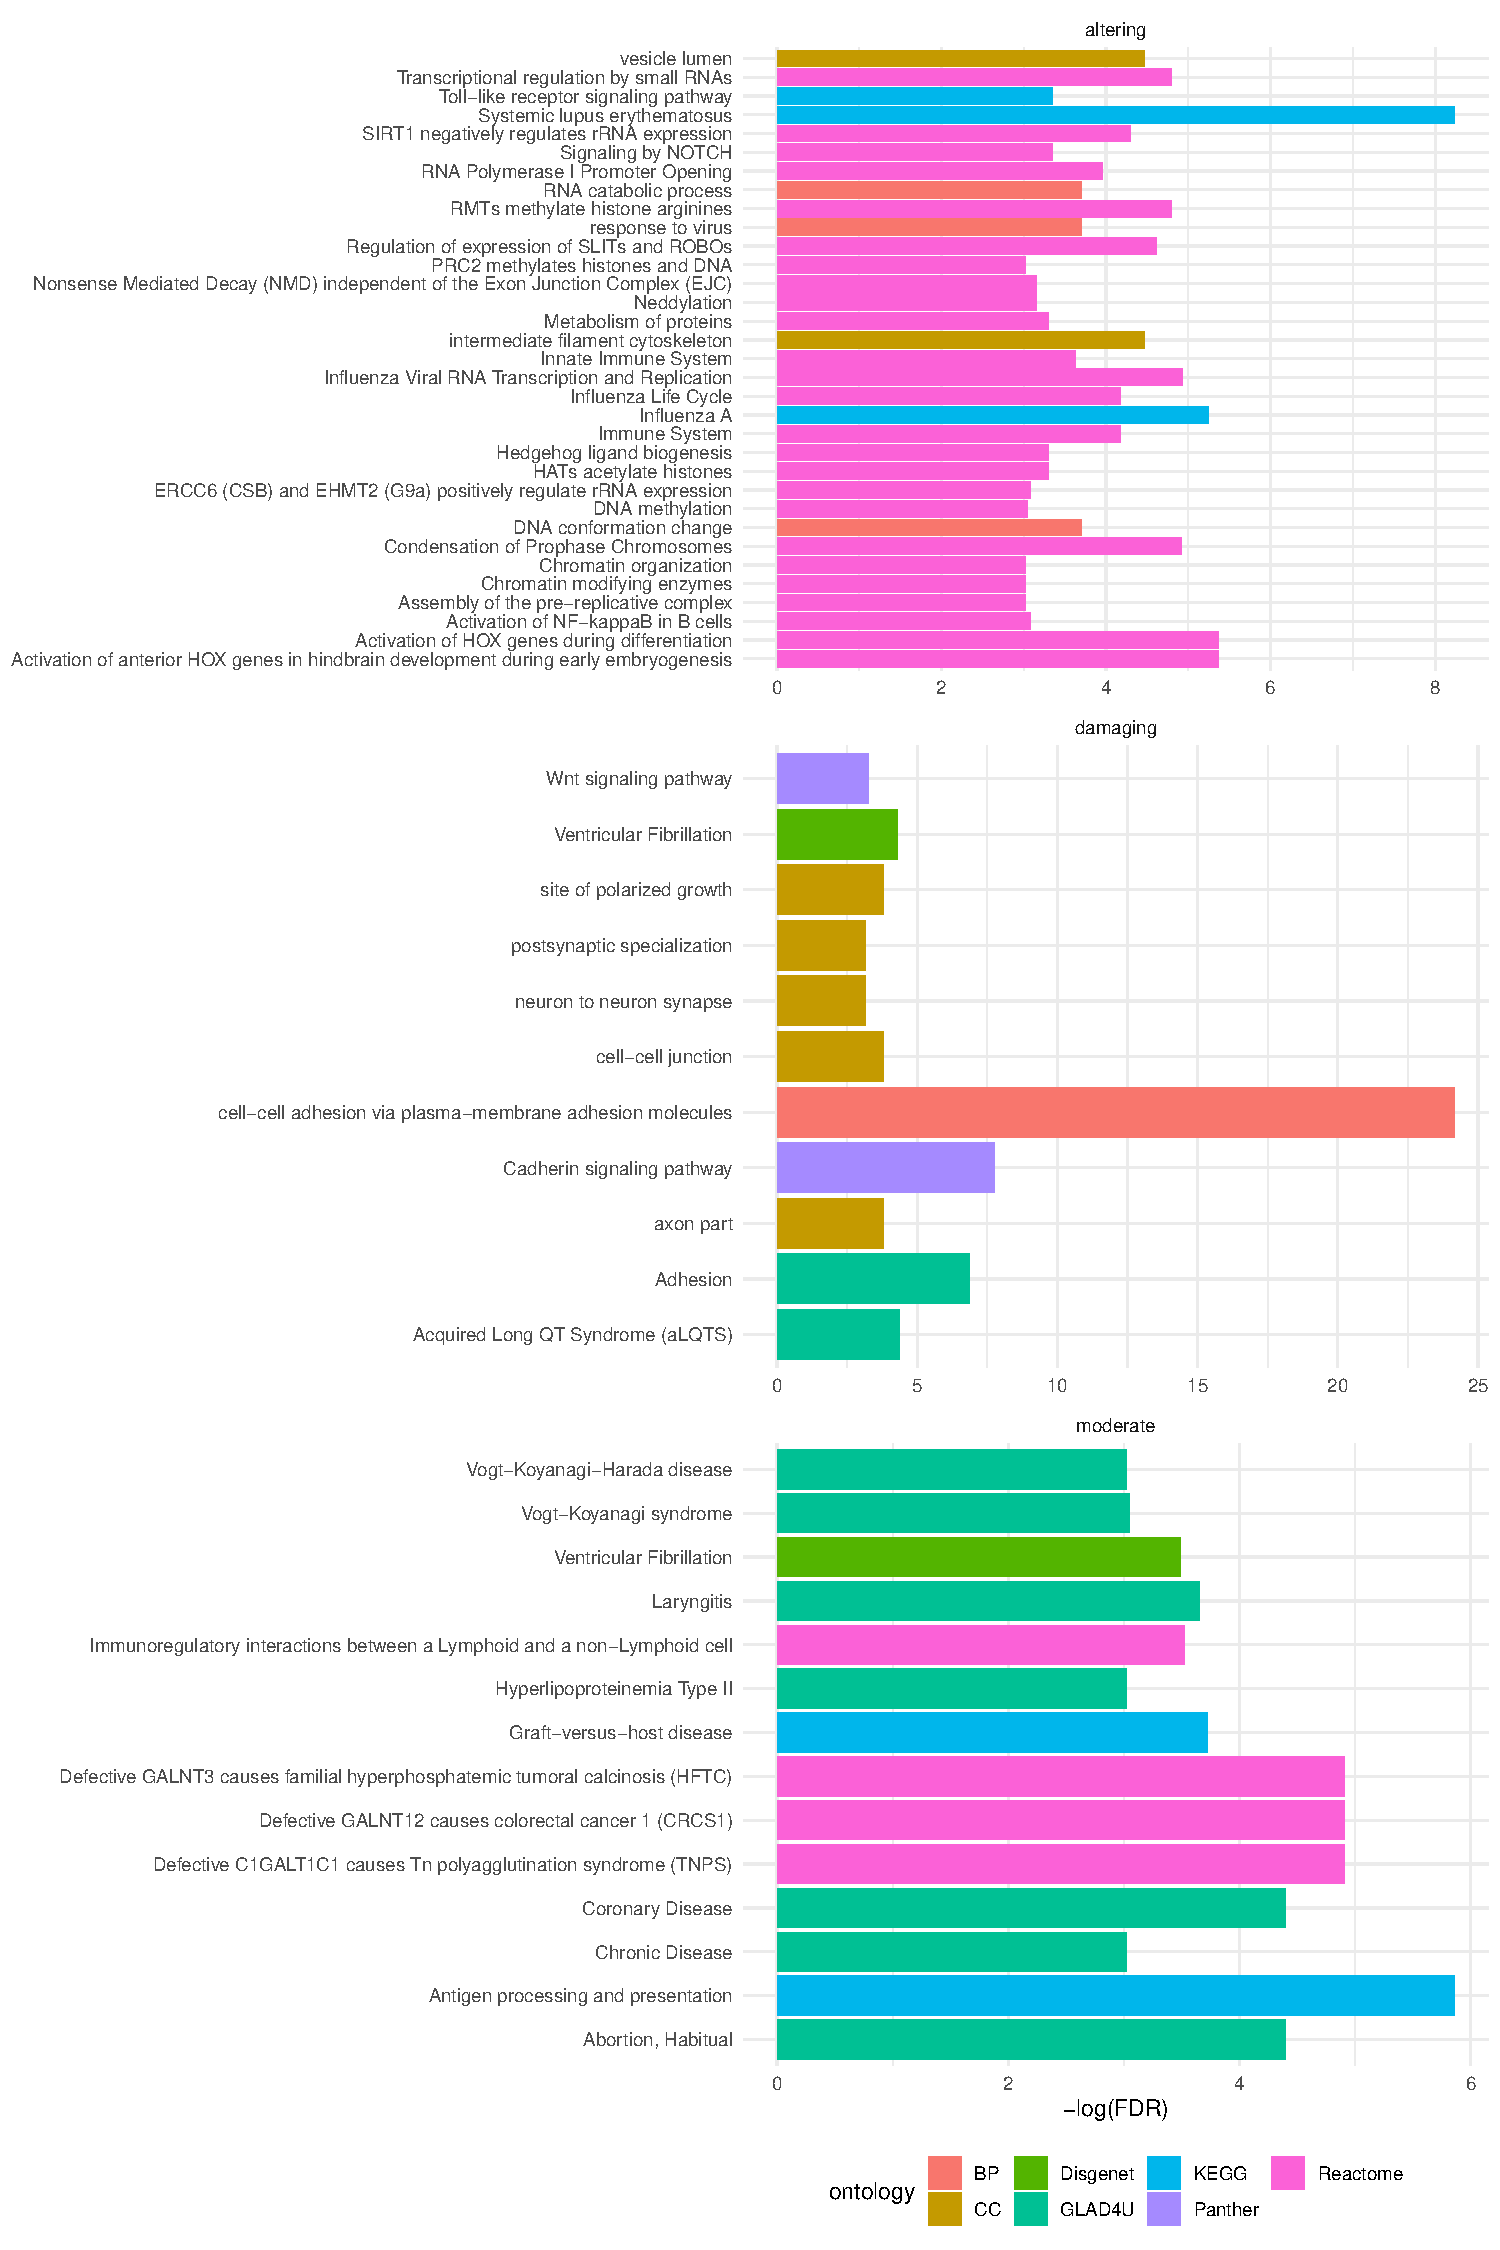
\includegraphics[totalheight=16cm]{barplot}
    %\caption{used by \citet[p.~4]{XXXXX}.}
    \caption{ORA results FDR $<$ 0.05.}
    \label{fig:ORA}
\end{figure}






% SECTION

\section{Hypothesis-free analysis: in search for novel target genes}
\label{sec:free}

A ``control set" of 76 1000G IBS women was considered. 1000G high coverage (30X) VCFs \href{REF}{REF} were filtered to SNVs and restricted to the ``control set" samples. All SNVs whereQUAL $>$ 20 and  FILTER is PASS were considered and the filtered VCFs were treated the same way as the described above for the Olot VCFs. 

The gene-level metrics of number and proportion of rare variants of interest in M116 (\autoref{sec:gene}) are compared with that of the ``control set"  (\textcolor{red}{TO BE FINISHED}).







% SECTION
\section{Remarkable findings}

\subsection{Immune genes}


ORA (\autoref{sec:fun}) found the many categories of the Immune System are enriched among the genes that harbour variants of interest, including.

\begin{itemize}
\item Immune System
\item Innate Immune System
\item Immunoregulatory interactions between a Lymphoid and a non\-Lymphoid cell
\item Antigen processing and presentation
\item Toll-like receptor signaling pathway
\item Systemic lupus erythematosus
\item Influenza A
\item response to virus
\end{itemize}

%Activation of anterior HOX genes in hindbrain development during early embryogenesis


%DNA
DNA conformation change
RNA catabolic process


\subsection{Bitter taste receptors}
% cat *.any.genes | grep grep TAS 
% cat *.altering.genes | grep TAS 
% (altering) TAS2R16 AND TAS2R5

Ventricular Fibrillation
Signaling by NOTCH

Bitter taste receptors have been associated with longevity \href{REF}{REF} and to cardiovascular morphology/function \cite{bloxham2020bitter}\cite{bloxham2024cardiac}, with a possible role in cardiac contractility and overall vascular tone.

The finding of variants of interest in TAS2R16 (only one statistically associated to longevity) and TAS2R5 is interesting in the light of the ORA results.



\subsection{Mitochondrial}

One mitochondrial rare variant of interest,, is associated to gene XXX. This gene is part of XXX machinery, associated with aging REF. 

% SECTION
\section{Conclusions}



% SECTION
%\section{References}

%\begin{thebibliography}{99} %99

\bibliography{supercentenarian_refs.bib}


%\end{thebibliography}



\end{document}




